\ifgerman{\chapter{Zukunftige Arbeiten}}{\chapter{Future Work}}
\label{futurework}

In this section, we describe ways to improve the visualization techniques that would help the user to improve their perception of the data presented. The general feedback presented \hyperref[sec:4.6]{Section 4.6} forms as a base for our future work.

Ratio plot as we know is a visual representation of configuration options and interaction with their general performance influence on the system. It does not present the information if performance influence was positive or negative. Hence, the most of the feedback from interviewees consisted of improved ratio plot which presents if the configuration option or interaction made a positive or a negative influence on the system. One way to achieve this, is to have an axis separating positive and negative influences. \hyperref[positiveNegative]{Figure 7.1}, shows a mock-up of the same.

\begin{figure}[ht]
\centering
\label{positiveNegative}
 %- \textbf{Your title}\par\medskip
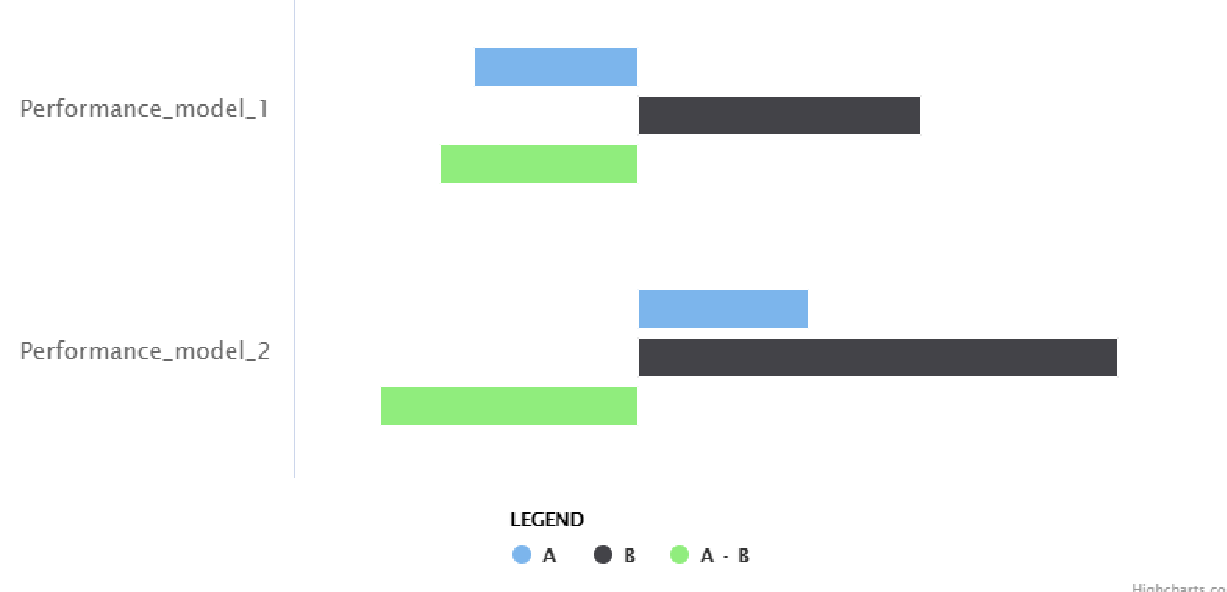
\includegraphics[width=15cm,height=15cm,keepaspectratio,]{pics/ratio_plot_with_positive_negative.pdf}
\caption[mockup1]{Mockup of ratio plot with configuration options A and B and interaction A $\cdot$ B for two performance-influence models, with separation between negative influences to the left side and positive influences to the right side of the center axis}
\end{figure}

Another improvement on ratio plot would be to show all the configuration options and interactions in the same order for all the performance-influence models. Currently, we display the configuration options and interactions in a sorted order from highest to lowest performance influence for each performance-influence model, which makes comparison a difficult task.  \hyperref[sameOrder]{Figure 7.2}, is a mock-up of the same.

\begin{figure}[ht]
\centering
\label{sameOrder}
 %- \textbf{Your title}\par\medskip
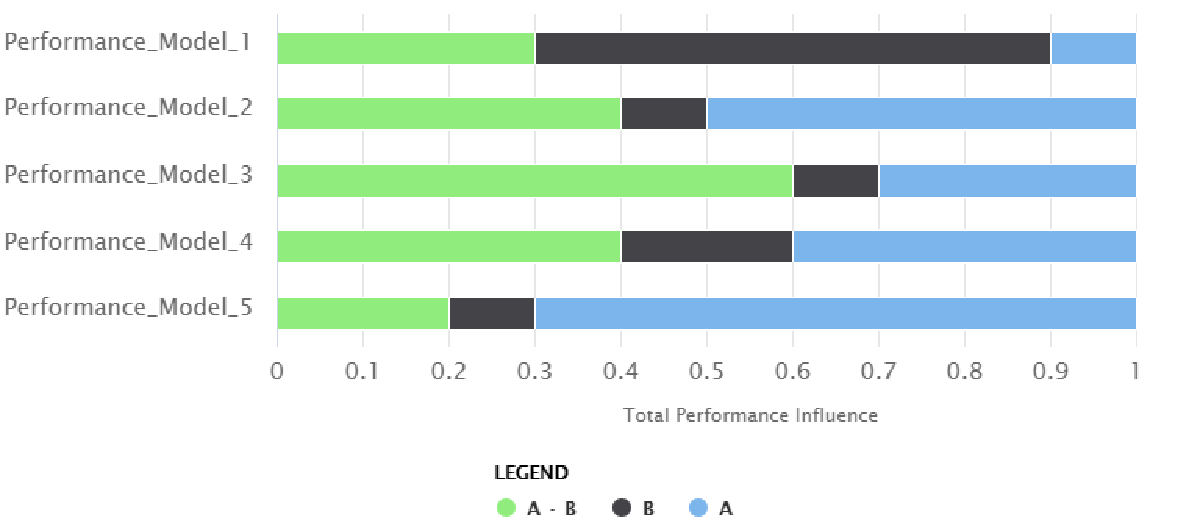
\includegraphics[width=15cm,height=15cm,keepaspectratio,]{pics/ratio_plot_without_sorted_order.pdf}
\caption[mockup2]{Mockup of ratio plot with configuration options A and B and interaction A $\cdot$ B of 5 performance-influence models all displayed in the same order}
\end{figure}


An improvement suggested for radar and text plot was to present the configuration options and interactions in a sorted order. This would help the users perception in finding the most relevant configuration option or interaction easily.

